
\documentclass[letterpaper,hide notes,xcolor={table,svgnames},pdftex,10pt]{beamer}
\def\showexamples{t}


%\usepackage[svgnames]{xcolor}

%% Demo talk
%\documentclass[letterpaper,notes=show]{beamer}

\usecolortheme{crane}
\setbeamertemplate{navigation symbols}{}

\usetheme{MyPittsburgh}
%\usetheme{Frankfurt}

%\usepackage{tipa}

\usepackage{hyperref}
\usepackage{graphicx,xspace}
\usepackage[normalem]{ulem}
\usepackage{multicol}
\usepackage{amsmath,amssymb,amsthm,graphicx,xspace}
\newcommand\SF[1]{$\bigstar$\footnote{SF: #1}}

\usepackage[default]{sourcesanspro}
\usepackage[T1]{fontenc}
\usepackage[scaled]{beramono}
\usepackage{tikzpagenodes}

\newcounter{tmpnumSlide}
\newcounter{tmpnumNote}


% old question code
%\newcommand\question[1]{{$\bigstar$ \small \onlySlide{2}{#1}}}
% \newcommand\nquestion[1]{\ifdefined \presentationonly \textcircled{?} \fi \note{\par{\Large \textbf{?}} #1}}
% \newcommand\nanswer[1]{\note{\par{\Large \textbf{A}} #1}}


 \newcommand\mnote[1]{%
   \addtocounter{tmpnumSlide}{1}
   \ifdefined\showcues {~\tiny\fbox{\arabic{tmpnumSlide}}}\fi
   \note{\setlength{\parskip}{1ex}\addtocounter{tmpnumNote}{1}\textbf{\Large \arabic{tmpnumNote}:} {#1\par}}}

\newcommand\mmnote[1]{\note{\setlength{\parskip}{1ex}#1\par}}

%\newcommand\mnote[2][]{\ifdefined\handoutwithnotes {~\tiny\fbox{#1}}\fi
% \note{\setlength{\parskip}{1ex}\textbf{\Large #1:} #2\par}}

%\newcommand\mnote[2][]{{\tiny\fbox{#1}} \note{\setlength{\parskip}{1ex}\textbf{\Large #1:} #2\par}}

\newcommand\mquestion[2]{{~\color{red}\fbox{?}}\note{\setlength{\parskip}{1ex}\par{\Large \textbf{?}} #1} \note{\setlength{\parskip}{1ex}\par{\Large \textbf{A}} #2\par}\ifdefined \presentationonly \pause \fi}

\newcommand\blackboard[1]{%
\ifdefined   \showblackboard
  {#1}
  \else {\begin{center} \fbox{\colorbox{blue!30}{%
         \begin{minipage}{.95\linewidth}%
           \hspace{\stretch{1}} Some space intentionally left blank; done at the blackboard.%
         \end{minipage}}}\end{center}}%
         \fi%
}



%\newcommand\q{\tikz \node[thick,color=black,shape=circle]{?};}
%\newcommand\q{\ifdefined \presentationonly \textcircled{?} \fi}

\usepackage{listings}
\lstset{basicstyle=\footnotesize\ttfamily,
	breaklines=true,
	aboveskip=15pt,
  	belowskip=15pt,
	frame=lines,
	numbers=left, basicstyle=\scriptsize, numberstyle=\tiny, stepnumber=0, numbersep=2pt
}

\usepackage{siunitx}
\newcommand\sius[1]{\num[group-separator = {,}]{#1}\si{\micro\second}}
\newcommand\sims[1]{\num[group-separator = {,}]{#1}\si{\milli\second}}
\newcommand\sins[1]{\num[group-separator = {,}]{#1}\si{\nano\second}}
\sisetup{group-separator = {,}, group-digits = true}

%% -------------------- tikz --------------------
\usepackage{tikz}
\usetikzlibrary{positioning}
\usetikzlibrary{arrows,backgrounds,automata,decorations.shapes,decorations.pathmorphing,decorations.markings,decorations.text,decorations.pathreplacing}

\tikzstyle{place}=[circle,draw=blue!50,fill=blue!20,thick, inner sep=0pt,minimum size=6mm]
\tikzstyle{transition}=[rectangle,draw=black!50,fill=black!20,thick, inner sep=0pt,minimum size=4mm]

\tikzstyle{block}=[rectangle,draw=black, thick, inner sep=5pt]
\tikzstyle{bullet}=[circle,draw=black, fill=black, thin, inner sep=2pt]

\tikzstyle{pre}=[<-,shorten <=1pt,>=stealth',semithick]
\tikzstyle{post}=[->,shorten >=1pt,>=stealth',semithick]
\tikzstyle{bi}=[<->,shorten >=1pt,shorten <=1pt, >=stealth',semithick]

\tikzstyle{mut}=[-,>=stealth',semithick]

\tikzstyle{treereset}=[dashed,->, shorten >=1pt,>=stealth',thin]

\usepackage{ifmtarg}
\usepackage{xifthen}
\makeatletter
% new counter to now which frame it is within the sequence
\newcounter{multiframecounter}
% initialize buffer for previously used frame title
\gdef\lastframetitle{\textit{undefined}}
% new environment for a multi-frame
\newenvironment{multiframe}[1][]{%
\ifthenelse{\isempty{#1}}{%
% if no frame title was set via optional parameter,
% only increase sequence counter by 1
\addtocounter{multiframecounter}{1}%
}{%
% new frame title has been provided, thus
% reset sequence counter to 1 and buffer frame title for later use
\setcounter{multiframecounter}{1}%
\gdef\lastframetitle{#1}%
}%
% start conventional frame environment and
% automatically set frame title followed by sequence counter
\begin{frame}%
\frametitle{\lastframetitle~{\normalfont(\arabic{multiframecounter})}}%
}{%
\end{frame}%
}
\makeatother

\makeatletter
\newdimen\tu@tmpa%
\newdimen\ydiffl%
\newdimen\xdiffl%
\newcommand\ydiff[2]{%
    \coordinate (tmpnamea) at (#1);%
    \coordinate (tmpnameb) at (#2);%
    \pgfextracty{\tu@tmpa}{\pgfpointanchor{tmpnamea}{center}}%
    \pgfextracty{\ydiffl}{\pgfpointanchor{tmpnameb}{center}}%
    \advance\ydiffl by -\tu@tmpa%
}
\newcommand\xdiff[2]{%
    \coordinate (tmpnamea) at (#1);%
    \coordinate (tmpnameb) at (#2);%
    \pgfextractx{\tu@tmpa}{\pgfpointanchor{tmpnamea}{center}}%
    \pgfextractx{\xdiffl}{\pgfpointanchor{tmpnameb}{center}}%
    \advance\xdiffl by -\tu@tmpa%
}
\makeatother
\newcommand{\copyrightbox}[3][r]{%
\begin{tikzpicture}%
\node[inner sep=0pt,minimum size=2em](ciimage){#2};
\usefont{OT1}{phv}{n}{n}\fontsize{4}{4}\selectfont
\ydiff{ciimage.south}{ciimage.north}
\xdiff{ciimage.west}{ciimage.east}
\ifthenelse{\equal{#1}{r}}{%
\node[inner sep=0pt,right=1ex of ciimage.south east,anchor=north west,rotate=90]%
{\raggedleft\color{black!50}\parbox{\the\ydiffl}{\raggedright{}#3}};%
}{%
\ifthenelse{\equal{#1}{l}}{%
\node[inner sep=0pt,right=1ex of ciimage.south west,anchor=south west,rotate=90]%
{\raggedleft\color{black!50}\parbox{\the\ydiffl}{\raggedright{}#3}};%
}{%
\node[inner sep=0pt,below=1ex of ciimage.south west,anchor=north west]%
{\raggedleft\color{black!50}\parbox{\the\xdiffl}{\raggedright{}#3}};%
}
}
\end{tikzpicture}
}


%% --------------------

%\usepackage[excludeor]{everyhook}
%\PushPreHook{par}{\setbox0=\lastbox\llap{MUH}}\box0}

%\vspace*{\stretch{1}

%\setbox0=\lastbox \llap{\textbullet\enskip}\box0}

\setlength{\parskip}{\fill}

\newcommand\noskips{\setlength{\parskip}{1ex}}
\newcommand\doskips{\setlength{\parskip}{\fill}}

\newcommand\xx{\par\vspace*{\stretch{1}}\par}
\newcommand\xxs{\par\vspace*{2ex}\par}
\newcommand\tuple[1]{\langle #1 \rangle}
\newcommand\code[1]{{\sf \footnotesize #1}}
\newcommand\ex[1]{\uline{Example:} \ifdefined \presentationonly \pause \fi
  \ifdefined\showexamples#1\xspace\else{\uline{\hspace*{2cm}}}\fi}

\newcommand\ceil[1]{\lceil #1 \rceil}


\AtBeginSection[]
{
   \begin{frame}
       \frametitle{Outline}
       \tableofcontents[currentsection]
   \end{frame}
}



\pgfdeclarelayer{edgelayer}
\pgfdeclarelayer{nodelayer}
\pgfsetlayers{edgelayer,nodelayer,main}

\tikzstyle{none}=[inner sep=0pt]
\tikzstyle{rn}=[circle,fill=Red,draw=Black,line width=0.8 pt]
\tikzstyle{gn}=[circle,fill=Lime,draw=Black,line width=0.8 pt]
\tikzstyle{yn}=[circle,fill=Yellow,draw=Black,line width=0.8 pt]
\tikzstyle{empty}=[circle,fill=White,draw=Black]
\tikzstyle{bw} = [rectangle, draw, fill=blue!20, 
    text width=4em, text centered, rounded corners, minimum height=2em]
    
    \newcommand{\CcNote}[1]{% longname
	This work is licensed under the \textit{Creative Commons #1 3.0 License}.%
}
\newcommand{\CcImageBy}[1]{%
	\includegraphics[scale=#1]{creative_commons/cc_by_30.pdf}%
}
\newcommand{\CcImageSa}[1]{%
	\includegraphics[scale=#1]{creative_commons/cc_sa_30.pdf}%
}
\newcommand{\CcImageNc}[1]{%
	\includegraphics[scale=#1]{creative_commons/cc_nc_30.pdf}%
}
\newcommand{\CcGroupBySa}[2]{% zoom, gap
	\CcImageBy{#1}\hspace*{#2}\CcImageNc{#1}\hspace*{#2}\CcImageSa{#1}%
}
\newcommand{\CcLongnameByNcSa}{Attribution-NonCommercial-ShareAlike}

\newenvironment{changemargin}[1]{% 
  \begin{list}{}{% 
    \setlength{\topsep}{0pt}% 
    \setlength{\leftmargin}{#1}% 
    \setlength{\rightmargin}{1em}
    \setlength{\listparindent}{\parindent}% 
    \setlength{\itemindent}{\parindent}% 
    \setlength{\parsep}{\parskip}% 
  }% 
  \item[]}{\end{list}} 





\title{Lecture 3 --- Rust: Borrowing, Slices, Threads, Traits  }

\author{Jeff Zarnett \\ \small \texttt{jzarnett@uwaterloo.ca}}
\institute{Department of Electrical and Computer Engineering \\
  University of Waterloo}
\date{\today}


\begin{document}

\begin{frame}
  \titlepage

 \end{frame}
 
 
\begin{frame}
\frametitle{Borrowing and References}

Ownership in Rust can come with unintended consequences, like accidentally giving away something we need later.

\begin{center}
	
\includegraphics[width=0.5\textwidth]{images/steve.jpeg}
\end{center}

Rust supports \alert{borrowing} -- you can use it but you promise you will give it back.

\end{frame}


\begin{frame}
\frametitle{Borrowing has rules}

Borrowing allows sharing in a controlled way.

The compiler analyzes borrowing with the \alert{borrow checker}. 

Its analysis always errs on the side of caution.


\end{frame}


\begin{frame}[fragile]
\frametitle{How to Borrow?}

The feature that we need for the concept of borrowing is the \alert{reference}.

The operator: \alert{\&}.

The reference operator appears both on the function definition and the invocation.

\begin{lstlisting}[language=Rust]
fn main() {
    let s1 = String::from("hello");
    let len = calculate_length(&s1);
    println!("The length of '{}' is {}.", s1, len);
}

fn calculate_length(s: &String) -> usize {
    s.len()
}
\end{lstlisting}

\end{frame}


\begin{frame}
\frametitle{Reference Rules}

The reference goes out of scope at the end of the function where it was used, removing it from consideration. 

A reference is not the same as ownership and the reference cannot exist without the original owner continuing to exist. 

\begin{center}
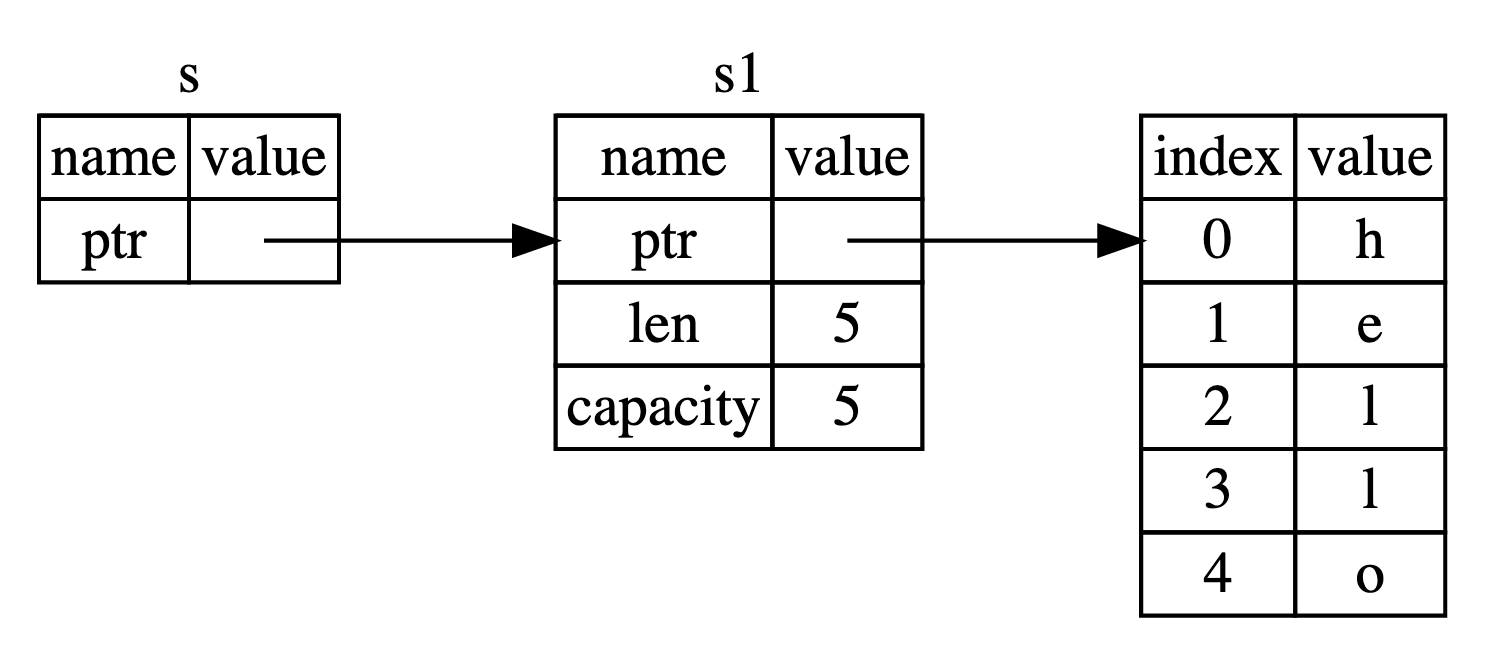
\includegraphics[width=0.6\textwidth]{images/string-with-ref.png}
\end{center}

\end{frame}


\begin{frame}[fragile]
\frametitle{Reference Rules}

If you borrow something, you can't do with it whatever you wish.

By default, you can't change it! 

Mutable references exist but must be explicitly declared:

\begin{lstlisting}[language=Rust]
fn main() {
    let mut s1 = String::from("hello");
    let len = calculate_length(&mut s1);
    println!("The length of '{}' is {}.", s1, len);
}

fn calculate_length(s: &mut String) -> usize {
    s.len()
}
\end{lstlisting}


\end{frame}


\begin{frame}
\frametitle{Mutable Reference Rules}

1. While a mutable reference exists, the owner can't change the data.

2. There can be only one mutable reference at a time.\\
\quad And when there is, no immutable references!

These restrictions prevent race conditions.

\end{frame}


\begin{frame}[fragile]
\frametitle{Time to Die}

References cannot outlive their underlying objects.

\begin{lstlisting}[language=Rust]
fn main() {
    let reference_to_nothing = dangle();
}

fn dangle() -> &String {
    let s = String::from("hello");
    &s
}
\end{lstlisting} 

In C this would be a ``dangling pointer''.

\end{frame}


\begin{frame}[fragile]
\frametitle{Non-Lexical Lifetimes}

A more recent improvement to Rust's borrow checking is called non-lexical lifetimes.

\begin{lstlisting}[language=Rust]
fn main() {
    let mut x = 5;

    let y = &x;
    println!("{}", y);

    let z = &mut x;
}
\end{lstlisting}

Under the old rules, the compiler would not allow creation of the mutable reference \texttt{z} because \texttt{y} has not gone out of scope.

\end{frame}


\begin{frame}
\frametitle{Slices}

The \alert{slice} concept exists in a few other programming languages, and if you have experience with them this will certainly help.

\begin{center}
	\includegraphics[width=0.25\textwidth]{images/pizza-slice.jpg}
\end{center}

A slice is a reference to a contiguous subset of the elements of a collection. 

\end{frame}


\begin{frame}[fragile]
\frametitle{A Less-Delicious Slice}

\begin{lstlisting}[language=Rust]
fn main() {
    let s = String::from("hello world");
    let hello = &s[0..5];
    let world = &s[6..11];
}
\end{lstlisting}

The representation of the slice looks like:
\begin{center}
	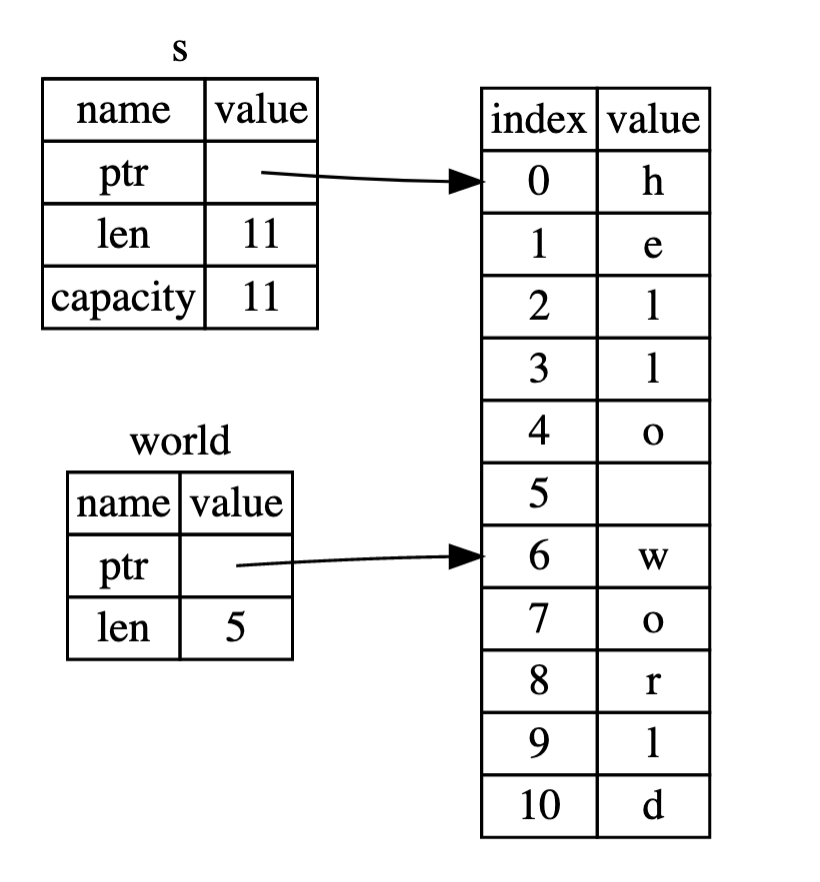
\includegraphics[width=0.4\textwidth]{images/string-slice.png}
\end{center}

\end{frame}


\begin{frame}
\frametitle{Why Slice?}

Slices can also apply to vectors and other collections, not just strings. 

As with the other kinds of references we've learned about, the existence of a slice prevents modification of the underlying data. 

Slices prevent race conditions on collections but also avoid (as much as possible) the need to copy data (slow).

\end{frame}


\begin{frame}
\frametitle{Unwrap Panic}

A lot of functions we use return \texttt{Result} types.


These return either \texttt{Ok} with the type we expected, or \texttt{Err} with an error description.

We must unpack the result.

Why?

\end{frame}



\begin{frame}
\frametitle{Unpack the Result}

If we try to open a file but the file doesn't exist, that's an error but one that's foreseeable and we can handle it. 

There's three ways to handle it: a \texttt{match} expression, \texttt{unwrap()}, and \texttt{expect()}. 


\end{frame}


\begin{frame}
\frametitle{Yikes!}

You may be tempted to just always use \texttt{unwrap()}

\begin{center}
	
\includegraphics[width=0.3\textwidth]{images/coyote.jpg}
\end{center}

Don't deny yourself the opportunity to add debug information.

It's better to use \texttt{expect()}.

\end{frame}


\begin{frame}
\frametitle{Plan for the Future}

It's recommended to use \texttt{Result} types for functions you write too. 

Make your future self happy by giving yourself the information you need to debug what's gone wrong!

This does come at a small performance hit. 

Remember though, your time (debugging) is valuable!

\end{frame}


\begin{frame}
\frametitle{Fearless Concurrency}

\begin{center}
	
\includegraphics[width=0.4\textwidth]{images/mindkiller.jpeg}
\end{center}

Rust is also intended to make concurrency errors compile-time problems too! 

As we know, concurrency brings new problems: race conditions, deadlock, etc.

Faster is not better if it makes your program incorrect.

\end{frame}

\begin{frame}
\frametitle{Fearless Concurrency}

A student in a previous term thought the Dune reference was too obscure.

\begin{center}
	
\includegraphics[width=0.6\textwidth]{images/fearless-concurrency.jpg}
\end{center}

\end{frame}


\begin{frame}
\frametitle{Wait, how does this help?}

If the compiler can help with making sure your concurrent program is correct, it doesn't make your program faster directly.

If you can be (more) sure of the correctness of your code, you don't have to spend as much time testing it.

Preventing a bug from being introduced is faster than finding and fixing it.

More guarantees help you write business-critical code with confidence.

\end{frame}


\begin{frame}
\frametitle{Threads}

Rust uses threads for concurrency, with a model that resembles the create/join semantics of the POSIX pthread. 

If you are unfamiliar with pthreads, the course repository has a PDF refresher of the topic (\texttt{pthreads.pdf}).

That PDF covers the POSIX thread in C, so you'll be on even footing.

\end{frame}


\begin{frame}[fragile]
\frametitle{So you want to create a thread...}

\begin{lstlisting}[language=Rust]
use std::thread;
use std::time::Duration;

fn main() {
    let handle = thread::spawn(|| {
        for i in 1..10 {
            println!("hi number {} from the spawned thread!", i);
            thread::sleep(Duration::from_millis(1));
        }
    });

    for i in 1..5 {
        println!("hi number {} from the main thread!", i);
        thread::sleep(Duration::from_millis(1));
    }

    handle.join().unwrap();
}
\end{lstlisting}

The thread being created takes as its argument a \alert{closure}.


The spawn call creates a \texttt{JoinHandle}.
\end{frame}


\begin{frame}
\frametitle{Too Easy}

This fails to capture the complexity of working with threads: no data is passed.

There are three ways that we can get data from one thread to another: capturing, message passing, and shared state.

\end{frame}


\begin{frame}[fragile]
\frametitle{Capture}

The notion of ``capturing'' calls back to the earlier mention that a closure captures some of its environment. 

\begin{lstlisting}[language=Rust]
use std::thread;

fn main() {
    let v = vec![1, 2, 3];

    let handle = thread::spawn(|| {
        println!("Here's a vector: {:?}", v);
    });

    handle.join().unwrap();
}
\end{lstlisting}

The only problem is: this example does not work.

The lifetime of \texttt{v} in the thread might outlive the scope creating the thread.

\end{frame}


\begin{frame}
\frametitle{What about Join?}

If I put something after the \texttt{join()} call that uses \texttt{v}, then the compiler should know that \texttt{v} has to remain in existence until after the thread in question. 

Yet, it still reports the error E0373 that says the thread might outlive the borrowed value. 

Turns out, I needed to understand \alert{lifetimes} in Rust better. We'll return to that.

\end{frame}


\begin{frame}
\frametitle{I like to move it}

Anyway, the error message suggests what you actually want in this scenario: to move the variables into the thread. 

Put \texttt{move} before the closure: \texttt{let handle = thread::spawn(move || \{}\ldots~ 

This addition results in the transfer of ownership to the thread being created. 

You can also copy if you need. 


\end{frame}


\begin{frame}
\frametitle{Don't Do It}

It might look like the error message is suggesting making the lifetime of your vector \texttt{static}.

\begin{center}
	
\includegraphics[width=0.3\textwidth]{images/stop-arnold.jpg}
\end{center}

Don't do it. We'll talk about why when we get into lifetimes.

\end{frame}


\begin{frame}
\frametitle{Message Passing}

Sometimes threads want to communicate in a way that isn't one-way communication at the time that the thread is being created.

Message passing may be familiar to you from previous courses.

Rust recommends this approach: harder to have races or invalid accesses.

\begin{center}
	
\includegraphics[width=0.5\textwidth]{images/sending-a-message.jpg}
\end{center}

\end{frame}


\begin{frame}
\frametitle{Ownership in Message Passing}

The ownership mechanic of message passing is like that of postal mail. 

So you want to have two threads communicate. 

The Rust metaphor for message-passing is called a \alert{channel}.\\
\quad It has a transmit-end and receive-end.

\end{frame}


\begin{frame}[fragile]
\frametitle{Communication Model}
The standard model is multiple-producer, single-consumer.

\begin{lstlisting}[language=Rust]
use std::sync::mpsc;
use std::thread;

fn main() {
    let (tx, rx) = mpsc::channel();

    thread::spawn(move || {
        let val = String::from("hi");
        tx.send(val).unwrap();
    });

    let received = rx.recv().unwrap();
    println!("Got: {}", received);
}
\end{lstlisting}

\texttt{recv()} is blocking and there is a corresponding \texttt{try\_recv()} 

We will cover non-blocking I/O soon.

\end{frame}


\begin{frame}
\frametitle{More About Sending}

If you want to have multiple transmitting ends, you need only use \texttt{clone} on the transmitter and hand those out as needed. 


As a small technical note, the type you want to send via a channel has to implement the \texttt{Send} trait.

But what is a trait? Let's talk about it.

\end{frame}


\begin{frame}[fragile]
\frametitle{Traits}

Traits are a lot like interfaces: you specify a set of function signatures.

To implement the trait, implement the functions.

\begin{lstlisting}[language=Rust]
pub trait FinalGrade {
	fun final_grade(&self) -> f32;
}

impl FinalGrade for Enrolled_Student {
    fn final_grade(&self) -> f32 {
        // Calculation of average according to syllabus rules goes here
    }	
}  
\end{lstlisting}

\end{frame}

\begin{frame}
\frametitle{Trait Rules}

You can only define traits on your own types.

You can create a default implementation.

Traits can be used as a return type or method parameter.\\
\quad Use the \texttt{+} to combine multiple traits in a parameter.

\end{frame}


\begin{frame}
\frametitle{The Big Three}

There are three traits that are really important to us right now. 

\texttt{Iterator}, \texttt{Send}, and \texttt{Sync}


\texttt{Iterator} is easy: put it on a collection, you can iterate over it.
\end{frame}


\begin{frame}
\frametitle{Send}

\texttt{Send} is used to transfer ownership between threads.

Some Rust types specifically don't implement Send as a way of saying, don't pass this between threads. 

If the compiler says no, you need a different type.

\end{frame}


\begin{frame}
\frametitle{Sync}

\texttt{Sync} means a type is thread-safe.


This does not mean all operations on a Sync type are safe and that no race conditions are possible.

If we need more than one thread to be able to modify the type, we need mutual exclusion.
\end{frame}


\begin{frame}
\frametitle{Back to the Mutex..}
There is also the ability to use a mutex.\\
\quad I assume you know how they work from previous courses.

New in Rust: the Mutex wraps a particular type.

It is defined as \texttt{Mutex<T>} and if you want an integer counter, you create it as \texttt{Mutex::new(0);}.


The Mutex goes with the value it is protecting.
\end{frame}


\begin{frame}[fragile]
\frametitle{Mutex In Action}

\begin{lstlisting}[language=Rust]
use std::sync::Mutex;

fn main() {
    let m = Mutex::new(5);

    {
        let mut num = m.lock().unwrap();
        *num = 6;
    }

    println!("m = {:?}", m);
}
\end{lstlisting}

You must acquire the mutex to access the internal value.

The lock operation returns a \texttt{MutexGuard}.\\
\quad When it goes out of scope, the lock is automatically unlocked.


\end{frame}


\begin{frame}
\frametitle{Silly Example}
This program has only one thread.

If we want to use it in multiple threads, we need multiple threads to access it. 

But we can't, unfortunately, just say that references will do! 

The mutex type has to outlive the other threads and such and the compiler will suggest moving it... 

But we can't move it into more than one thread, because that violates our rule about having only one owner. 

What now?



\end{frame}

\begin{frame}
\frametitle{Breaking the Law, Breaking the Law}

\begin{center}
	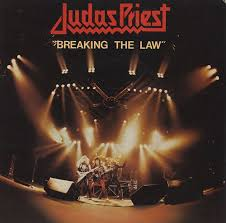
\includegraphics[width=0.5\textwidth]{images/judaspriest.jpg}
\end{center}

We have to break a rule: we need to share ownership of some memory. 

\end{frame}


\end{document}

